%
% Samuel Plaça de Paula, 2012
% http://www.linux.ime.usp.br/~samuel/mac499/
% samuplaza@gmail.com
%
% Baseado no exemplo disponibilizado por Jesús P. Mena-Chalco:
%
% poster-exemplo (versão minimalista)
% http://www.vision.ime.usp.br/~jmena/stuff/poster-exemplo/
%

\documentclass[final]{beamer} 
\usepackage[size=custom,width=70.7,height=100,scale=1.0]{beamerposter} % font scale factor=1.0

\usepackage[brazil]{babel}
\usepackage[utf8]{inputenc}

% para poder usar imagens eps e psfrag

%\usepackage{epstopdf} 
%\usepackage{epsfig}
\usepackage{graphicx}
\newcommand{\tdots}{\,.\,.\,} % in place of \ldots

\usepackage{tikz}
\usepackage{tikz-qtree}
\usetikzlibrary{matrix,backgrounds, decorations.pathreplacing, automata, arrows}
\usepackage{subfig}



\newcommand{\E}{\Sigma}
\newcommand{\cS}{\mathcal{S}}
\newcommand{\Oh}{\mathcal{O}}
\renewcommand{\emph}[1]{\textbf{#1}}


\newcommand{\PP}{\mbox{P}}
\newcommand{\NP}{\mbox{NP}}
\newcommand{\PL}{\mathit{PL}}
\newcommand{\PLI}{\mathit{PLI}}
\newcommand{\OPT}{\mbox{OPT}}

\newtheorem{teo}{Teorema}[section]  % numerado por section
\newtheorem{lema}[teo]{Lema}        % numerado como teo
\newtheorem{cor}[teo]{Corolário}    % numerado como teo
\newtheorem{fato}[teo]{Fato}        % numerado como teo
\newtheorem{mdef}[teo]{Definição}   % numerado como teo

\newcommand{\emptystring}{\varepsilon}

%cardinalidade
\newcommand{\card}[1]
{\left|#1\right|}

\let\:=\colon
\let\epsilon=\varepsilon

\def\({\left(}
\def\){\right)}
\def\<{\langle}
\def\>{\rangle}

% valor (e.g., de uma solução)
\newcommand{\Val}[1]
{\mathrm{val}\(#1\)}


% cores utilizadas para os algoritmos
\usepackage{framed}
\definecolor{azul}{rgb}{0.76471,0.81176,0.91373}  % c3cfe9 -> 195,207,233 -> 0.76471   0.81176   0.91373
\definecolor{lilas}{rgb}{0.83529,0.80784,0.89804} % d5cee5 -> 213,206,229 -> 0.83529   0.80784   0.89804
\definecolor{ops}{rgb}{0.9,0.9,0.9} % d5cee5 -> 213,206,229 -> 0.83529   0.80784   0.89804

\urlstyle{same}

%==The poster style============================================================
\usetheme{poster-exemplo}            % our poster style
%--set colors for blocks (without frame)---------------------------------------
  \setbeamercolor{block title}{fg=dblue,bg=white}
  \setbeamercolor{block body}{fg=black,bg=white}
%--set colors for alerted blocks (with frame)----------------------------------
%--textcolor = fg, backgroundcolor = bg, dblue is the jacobs blue
  \setbeamercolor{block alerted title}{fg=dblue,bg=gray!50}%frame color
  \setbeamercolor{block alerted body}{fg=black,bg=gray!20}%body color
%
%==Title, date and authors of the poster=======================================
\title{Algoritmos em sequências}
\author{Yan Soares Couto \hspace{100pt} Orientadora: Cristina Gomes Fernandes}
\institute{\vspace{10pt}Departamento de Ciência da Computação,
Instituto de Matemática e Estatística, Universidade de São Paulo}
%\date{\today}


%==============================================================================
%==the poster content==========================================================
%==============================================================================
\begin{document}
%--the poster is one beamer frame, so we have to start with:
\begin{frame}[t]
%--to seperate the poster in columns we can use the columns environment
\begin{columns}[t] % the [t] options aligns the columns content at the top
%--the left column-------------------------------------------------------------
%\begin{column}{0.28\paperwidth}% the right size for a 3-column layout
\begin{column}{0.35\paperwidth}% the right size for a 3-column layout

	\begin{alertblock}{Introdução}


O crescimento expressivo na capacidade de armazenamento 
de dados em meios digitais criou a demanda por algoritmos 
cada vez mais eficientes para realizar buscas por padrões em 
textos.  Dependendo da situação tais buscas podem ser por 
ocorrências exatas ou por ocorrências aproximadas do padrão. \vskip2ex

Algoritmos de busca de padrão têm aplicação não só em 
atividades do nosso dia a dia, quando frequentemente usamos, 
em um editor ou em um browser, comandos de busca por um 
padrão, como também por exemplo em problemas de biologia 
computacional, quando buscamos padrões em sequências de 
DNA ou de proteína. \vskip2ex

Algoritmos clássicos como o KMP e o Boyer-Moore são abordados 
em disciplinas de um curso de graduação em Ciência da Computação. 
Nesse trabalho, abordamos algoritmos e estruturas de dados mais 
sofisticados e poderosos, que resolvem não apenas um problema 
específico de busca, mas uma classe de problemas, de maneira eficiente.	


%Encontrar todas as ocorrências de uma certa palavra em um texto é um problema muito importante, que vemos diariamente, por exemplo ao buscar uma palavra-chave em seus emails recebidos, ou ao usar a função do \texttt{CTRL-F} em algum documento. \vskip2ex

%Algoritmos desse tipo resolvem problemas de busca de ocorrências exatas, quando não são aceitas diferenças entre o padrão buscado e as posições de ocorrência retornadas. Outra classe de problemas é de busca de ocorrências inexatas, ou busca de ocorrências aproximadas, quando algumas diferenças são aceitas. Nesse caso é necessário adotar alguma definição de similaridade entre duas cadeias de caracteres, em geral o número mínimo de caracteres que precisam ser mudados para tornar ambas cadeias iguais. O utilitário \texttt{diff}, por exemplo, encontra o número mínimo de linhas que precisam ser mudadas para tornar dois arquivos iguais.  \vskip2ex
%
%Outra área que se beneficia do desenvolvimento desses algoritmos é a área da biologia computacional, pois DNA pode ser modelado como uma sequência de caracteres \texttt{A}, \texttt{T}, \texttt{C} e \texttt{G}. Assim, é possível encontrar similaridades entre trechos de DNAs diferentes, e buscar, em um conjunto enorme de trechos de DNA, algum similar ou idêntico a um trecho dado. Proteínas também podem ser modeladas como uma sequência de aminoácidos.  \vskip2ex

	\end{alertblock}
	\vskip2ex

	\begin{block}{Objetivos}

Estudo e implementação de algoritmos sofisticados e eficientes para  problemas de busca de padrão e variantes. \vskip2ex

Apresentação tão completa e didática quanto possível dos algoritmos e estruturas de dados estudados.  Disponibilização das implementações desenvolvidas no github. 

\definecolor{shadecolor}{named}{azul}
\begin{shaded}

Dado um alfabeto $\E$, uma string~$T$ é uma sequência finita de símbolos de~$\E$. Defina~$T[i]$ como o $i$-ésimo símbolo dessa sequência. \vskip2ex

Dizemos que~${T[i\tdots j] = T[i] T[i+1] \ldots T[j]}$ é uma \emph{substring} de~$T$.

\begin{figure}
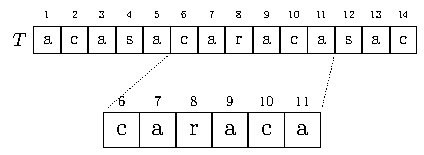
\includegraphics[scale=2.2]{substr.pdf}
\end{figure}



Um prefixo de~$T$ é uma substring que começa na posição~$1$, e um sufixo de~$T$ é uma substring que termina na posição~$|T|$.
Dizemos que $T_1$ ocorre em~$T_2$ se~$T_1$ é uma substring de~$T_2$.
\end{shaded}

%Neste trabalho, desenvolvemos algoritmos e estruturas de dados relacionados aos problemas de busca de ocorrências exatas. Os algoritmos clássicos para encontrar ocorrências exatas, como KMP e Boyer-Moore, não são abordados. O foco é em estruturas mais poderosas, que generalizam os algoritmos clássicos, são mais rápidos ou resolvem problemas mais difíceis, apesar de serem mais complicados. \vskip2ex
%
%Diferentemente dos livros e fontes mais comuns, a implementação é bastante discutida, com pseudocódigo usando apenas instruções presentes nas principais linguagens de programação. Porém, a teoria não é esquecida. Ao apresentar os algoritmos e suas explicações, a corretude e complexidade são provadas formalmente, sem grandes pulos de lógica e sem uso de resultados complicados que não estão provados no texto.
%


	\end{block}
    \vskip2ex

    \begin{block}{Tries}
    
Uma trie é uma estrutura de dados que armazena um conjunto de strings~$\cS$. \vskip2ex

  \setbeamercolor{block alerted title}{fg=black,bg=gray!20}%frame color
  \setbeamercolor{block alerted body}{fg=black,bg=white}%body color
\begin{alertblock} {Operações}
\begin{description}
\item [\textsc{Contains}$(P)$:] Determina se~$P \in \cS$. Tempo~$\Oh(|P|)$. \vskip1ex
\item [\textsc{LCP}$(P)$:] Retorna o maior prefixo comum de~$P$ com \emph{alguma} string de~$\cS$. Tempo~$\Oh(|P|)$.
\end{description}
\end{alertblock}
\vskip2ex

\begin{figure}
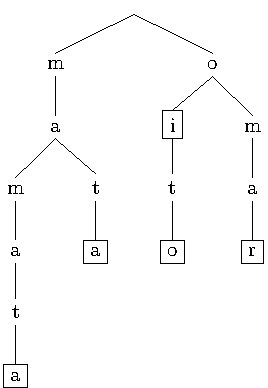
\includegraphics[scale=2]{trie_ex.pdf}
\caption{Uma trie exemplo para~$\cS = $\{mamata, mata, oi, oito, omar\}.}
\end{figure}

A imagem ilustra uma trie. Os vértices marcados indicam os fins das strings no conjunto. É possível construir uma trie para~$\cS = \{S_1, \ldots, S_k\}$ em tempo~$\Oh(\sum\limits_{i = 1}^k{|S_i|} \cdot |\E|)$. \vskip2ex

    \end{block}

% ---------------------------------------------------------------------------- %

	\begin{block}{Informações e contato}
        Para mais informações, acesse a página do trabalho:

		\textcolor{jblue}{{\url{http://www.linux.ime.usp.br/~yancouto/mac0499}}}
        \vskip2ex
        Endereço para contato: \textcolor{jblue}
        {{\url{yancouto@ime.usp.br}}}

	\end{block}

\end{column}


% ---------------------------------------------------------------------------- %
\begin{column}{0.60\paperwidth} 
	\begin{block}{Estruturas em tries}

É possível guardar algumas informações adicionais na trie, ou usar uma forma diferente de armazená-la, para torná-la ainda mais poderosa. Estas versões alternativas são úteis para busca de ocorrências exatas de conjuntos.

		\begin{columns}[c,totalwidth=0.60\paperwidth]

		\begin{column}{0.47\columnwidth}
		\begin{block}{Aho-Corasick}

Para um conjunto~$\cS = \{S_1, \ldots, S_k\}$ de strings, após preprocessamento na trie para~$\cS$, é possível realizar: \vskip1ex

  \setbeamercolor{block alerted title}{fg=black,bg=gray!20}%frame color
  \setbeamercolor{block alerted body}{fg=black,bg=white}%body color
\begin{alertblock} {Operações}
\begin{description}
\item [\textsc{Any}$(P)$:] Determina se alguma string de~$\cS$ ocorre em~$P$. Tempo~$\Oh(|P|)$. \vskip1ex
\item [\textsc{Count}$(P)$:] Para cada string~$S_i \in \cS$, determina o número de ocorrências de~$S_i$ em~$P$. Tempo~$\Oh(|P| + \sum\limits_{i=1}^k{|S_i|})$.
\end{description}
\end{alertblock}
\vskip1ex

Para cada vértice~$u$, o seu \emph{link de falha} é o nó mais profundo cuja string é um sufixo próprio da string associada a~$u$. Note que essa ideia é uma generalização da função prefixo calculada no algoritmo KMP.

\begin{figure}
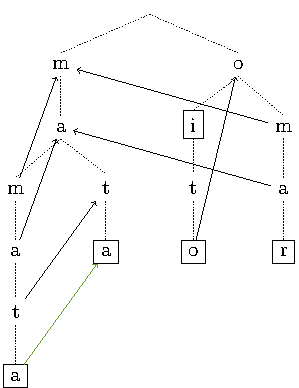
\includegraphics[scale=2]{linkfalha_ex.pdf}
\caption{Links de falha para a trie exemplo. Os links para a raiz foram omitidos.}
\end{figure}

O \emph{link de ocorrência} de~$u$ é o nó que representa a maior string de~$\cS$ que é sufixo próprio da string associada a~$u$.
O link destacado na figura é o único link de ocorrência. \vskip2ex

A estrutura e algoritmo apresentado foi criado por Alfred V. Aho e Margaret J. Corasick \cite{aho}.

        \end{block}
        \end{column}

		\begin{column}{0.5\columnwidth}
		\begin{block}{Árvore de Sufixos}

Uma árvore de sufixos é uma trie para todos os sufixos de~$S$. \vskip2ex
		
\setbeamercolor{block alerted title}{fg=black,bg=gray!20}%frame color
\setbeamercolor{block alerted body}{fg=black,bg=white}%body color
\begin{alertblock} {Operações}
\begin{description}
\item [\textsc{Count}$(P)$:] Determina o número de ocorrências de~$P$ em~$S$. Tempo~$\Oh(|P|)$.
\item [\textsc{List}$(P)$:] Retorna uma lista com as posições de todas as ocorrências de~$P$ em~$S$. Tempo~$\Oh(|P| + x)$, onde~$x$ é o número de tais ocorrências.
\end{description}
\end{alertblock}
\vskip1ex

Comprimindo vértices que têm apenas um filho, o número de vértices da trie fica no máximo~$2|S|$.

\begin{figure}
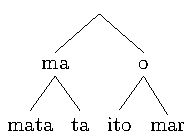
\includegraphics[scale=2.5]{triecompr.pdf}
\caption{Trie comprimida para~$T$}
\end{figure}

É possível construir esta árvore de sufixos em tempo e espaço~$\Oh(|S||\E|)$.

\begin{figure}
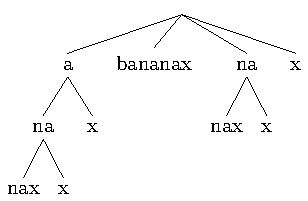
\includegraphics[scale=2.5]{sufftree.pdf}
\caption{Árvore de sufixos de \texttt{bananax}.}
\end{figure}

O primeiro algoritmo para criação de árvores de sufixos em tempo linear foi proposto por Weiner~\cite{weiner}, mas o algoritmo apresentado no texto é de Ukkonen~\cite{ukkonen}.

        \end{block}
		\end{column}
		\end{columns}

	\end{block}
	%\vskip2ex

\vskip2ex

% ---------------------------------------------------------------------------- %
\begin{block}{Autômato de Sufixos}

Autômato de sufixos é um autômato que reconhece todos os sufixos de uma string~$S$. \vskip1ex

\setbeamercolor{block alerted title}{fg=black,bg=gray!20}%frame color
\setbeamercolor{block alerted body}{fg=black,bg=white}%body color
\begin{alertblock} {Operações}
\begin{description}
\item [\textsc{Count}$(P)$:] Determina o número de ocorrências de~$P$ em~$S$. Tempo~$\Oh(|P|)$.
%\item [\textsc{Occs}$(P)$:] Retorna uma lista com as posições de todas as ocorrências de~$P$ em~$S$. Tempo~$\Oh(|P| + x)$, onde~$x$ é o número de tais ocorrências.
\end{description}
\end{alertblock}
\vskip1ex

Cada nó em um autômato de sufixos identifica um conjunto de ocorrências à direita. \vskip1ex

${D(P) = \{i : P\text{ é sufixo de } S[1\tdots i]\}}$ é o conjunto de ocorrências à direita de~$P$. \vskip1ex

\begin{figure}
\subfloat[$\emptystring$] {
\begin{minipage}{0.3\columnwidth}
\centering
\hspace{-1.6cm}
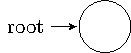
\includegraphics[scale=1.2]{empty.pdf}
\end{minipage}
}
\hfill
\subfloat[b] {
\begin{minipage}{0.3\columnwidth}
\hspace{-1.5cm}
\centering
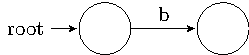
\includegraphics[scale=1.2]{b.pdf}
\end{minipage}
}
\hfill
\subfloat[ba] {
\begin{minipage}{0.35\columnwidth}
\centering
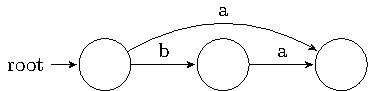
\includegraphics[scale=1.2]{ba.pdf}
\end{minipage}
}
\hfill
\subfloat[ban] {
\begin{minipage}{0.3\columnwidth}
\centering
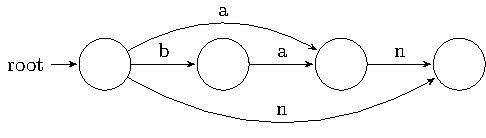
\includegraphics[scale=1.2]{ban.pdf}
\end{minipage}
}
\hfill
\subfloat[bana] {
\begin{minipage}{0.3\columnwidth}
\centering
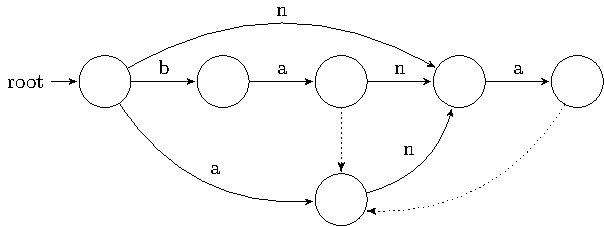
\includegraphics[scale=1.2]{bana.pdf}
\end{minipage}
}
\hfill
\subfloat[banan] {
\begin{minipage}{0.35\columnwidth}
\centering
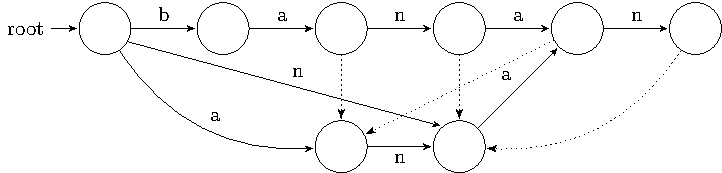
\includegraphics[scale=1.2]{banan.pdf}
\end{minipage}
}
\hfill
\subfloat[banana]{
\begin{minipage}{\columnwidth}
\centering
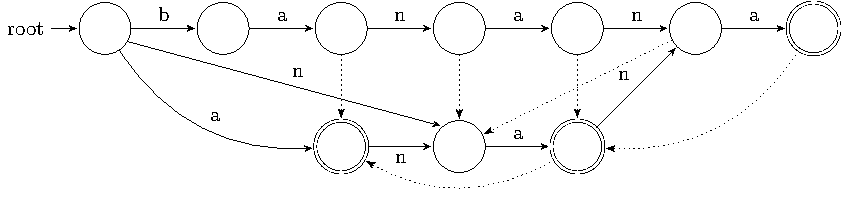
\includegraphics[scale=1.9]{banana.pdf}
\end{minipage}
}

\caption{Construção do autômato de sufixos de \texttt{banana}, falhas desenhadas pontilhadas.}
\end{figure}

O número de vértices do autômato é no máximo~$2|S|$. A estrutura tem usos bem similares aos da árvore de sufixos, mas a implementação é mais simples. \vskip2ex

O \emph{link de falha} de um nó aponta para o nó cujo conjunto de ocorrências à direita o contém propriamente.

%O digrafo tem um vértice chamado de raiz, e cada aresta está associada a um caractere. O caminho a partir da raiz pela string~$P$ termina no vértice que representa~$D(P)$. Note que caminhos diferentes podem acabar no mesmo vértice. \vskip1ex
%
%O conjunto $V = \{D(P) : P\text{ ocorre em } S\}$, de vértices do autômato, e de conjuntos de ocorrências à direita, é laminar, ou seja, para todo~$a, b \in V$, vale que~$a \cap b = \emptyset$,~$a \subseteq b$ ou~$b \subseteq a$.
%
%Dessa forma, pode-se provar que o número de vértices do autômato é no máximo~$2 |S|$.
%É possível construir o autômato em tempo linear, usando que, ao adicionar um caractere em~$S$, o número de conjuntos em~$V$ aumenta em no máximo~2, e apenas um conjunto ``se separa''. \vskip2ex
%        
%
%A estrutura do autômato de sufixos é muito menos intuitiva que a árvore de sufixos, mas seus usos são bem similares, e o código para este é mais simples.
%Para descobrir se~$P$ ocorre em~$S$, basta determinar se é possível percorrer o caminho indexado por~$P$ a partir da raiz.

\end{block}
\vspace{-1ex}
\begin{block}{Referências}
	\scriptsize{\begin{thebibliography}{99}
	\bibitem{aho}
    Aho, Alfred V. and Corasick, Margaret J.,
	``\textbf{Efficient string matching: an aid to bibliographic search},'' in \textit{Commun. ACM}, 1975, 18 (6), pp. 333–340.

    \bibitem{weiner}
    Peter Weiner,
    ``\textbf{Linear pattern matching algorithms},'' in \textit{14th Symposium on Switching and Automata Theory}, 1973.

    \bibitem{ukkonen}
    Ukkonen, Esko,
    ``\textbf{On-line construction of suffix trees}'', in \textit{Algorithmica}, 1995, 14 (3), pp. 249–260.

	\end{thebibliography}}
%\hfill{\includegraphics[height=6cm]{logo-ime.svg}}
\end{block}

\end{column}

\end{columns}
% ---------------------------------------------------------------------------- %
\end{frame}
\end{document}
